\documentclass[11pt]{beamer}
\usetheme{Warsaw}
\usepackage[utf8]{inputenc}
\usepackage[spanish]{babel}
\usepackage{amsmath}
\usepackage{amsfonts}
\usepackage{amssymb}
\usepackage{graphicx}
\usepackage{multicol}


% Datos
\author{N.Pérez-Medina$^1$, Dr.José L.Herrera-Aguilar$^2$}
\title{\textbf{Análisis estadístico de características musicales de la salsa.}}
\setbeamercovered{transparent} 
\setbeamertemplate{navigation symbols}{} 
\logo{
\includegraphics[scale=0.05]{logo_fing_uach_bn.png} } 
\institute{
			\textbf{Avance de tesis de licenciatura} \\
			\medskip
			$^1$Estudiante de Ingeniería Matemática.\\
			$^2$Laboratorio de Sistemas Complejos. \\
			Facultad de Ingeniería, UACH.\\
			\bigskip
			\begin{small}
			\textit{\textbf{58 Congreso Nacional de la Sociedad Matemática Mexicana}}\\	
			\end{small}
			
	} 
\date{} 


% Para tener un morado coqueto
\definecolor{lightPurple}{RGB}{186, 146, 209} % Morado claro
\definecolor{darkPurple}{RGB}{98, 54, 150}    % Morado oscuro
\setbeamercolor{structure}{fg=darkPurple} % Color principal para estructuras
\setbeamercolor{frametitle}{bg=darkPurple, fg=white} % Título del marco
\setbeamercolor{block title}{bg=darkPurple, fg=white} % Título de bloques
\setbeamercolor{block body}{bg=lightPurple!30, fg=black} % Cuerpo de bloques




\begin{document}

\begin{frame}
\titlepage
\end{frame}

\begin{frame}
\tableofcontents
\end{frame}

\section{Contextualización}
\subsection{Objetivo general}
\begin{frame}
\tableofcontents[currentsection] % Solo muestra la sección actual
\end{frame}

\begin{frame}{¿Qué pretendemos hacer?}
	\begin{block}{\textbf{Objetivo general}}
		Caracterizar géneros musicales mediante el análisis estadístico de las \textit{propiedades musicales} para generar una \textbf{base cuantitativa que permita determinar la pertenencia de una canción a un género musical específico.}
	\end{block}
	\centering
	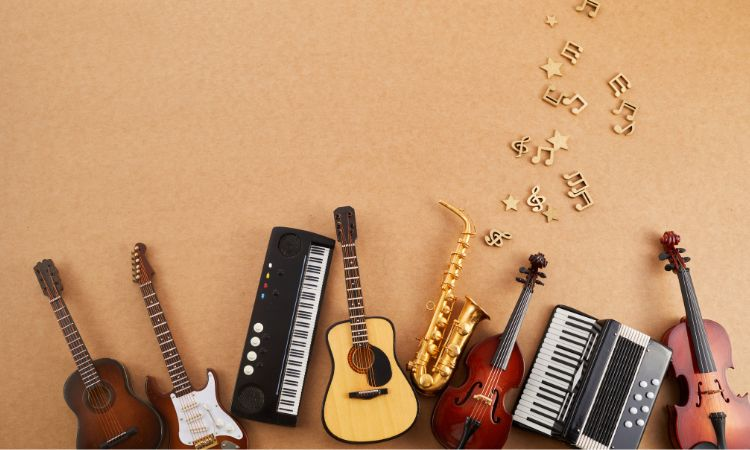
\includegraphics[scale=0.3]{estilos-musicales-diferencias.jpg} 
\end{frame}

\subsection{Marco Teórico}


\subsubsection*{Enciclopedia musical - \textit{MusicBrainz}}
\begin{frame}{\textit{MusicBrainz}}
	\begin{block}{\textbf{En general}}
		\begin{itemize}
			\item Creada en el 2000 por \textbf{Robert Kaye.}
			\item Metadatos de \textbf{más de 4.7 millones de lanzamientos}
			\item Sistema de etiquetas y votación comunitaria.
			\item Permite consultar mediante su \textbf{API}.
		\end{itemize}
	\end{block}
	\centering
	
\includegraphics[scale=.5]{musicbrainz.png} 
\end{frame} 


\subsubsection*{Archivos MIDI}
\begin{frame}{Sobre los archivos \textbf{MIDI}}
\begin{block}{\textbf{M}usical \textbf{I}nstrument \textbf{D}igital \textbf{I}nterface}
\textbf{MIDI} es un \textit{''protocolo digital''} que no almacena audio sino:
\begin{itemize}
\item Qué \textbf{instrumento} tocar
\item En qué momento tocar cierta \textbf{nota}
\item \textbf{Cuánto tiempo} y a qué \textbf{volumen} tocar esa nota
\end{itemize}
\end{block}

\begin{block}{Esto nos permite}
Visitar esos datos y reconstruir un mapa temporal muy detallado de una canción
\end{block}
\end{frame}

\begin{frame}{Idea gráfica}

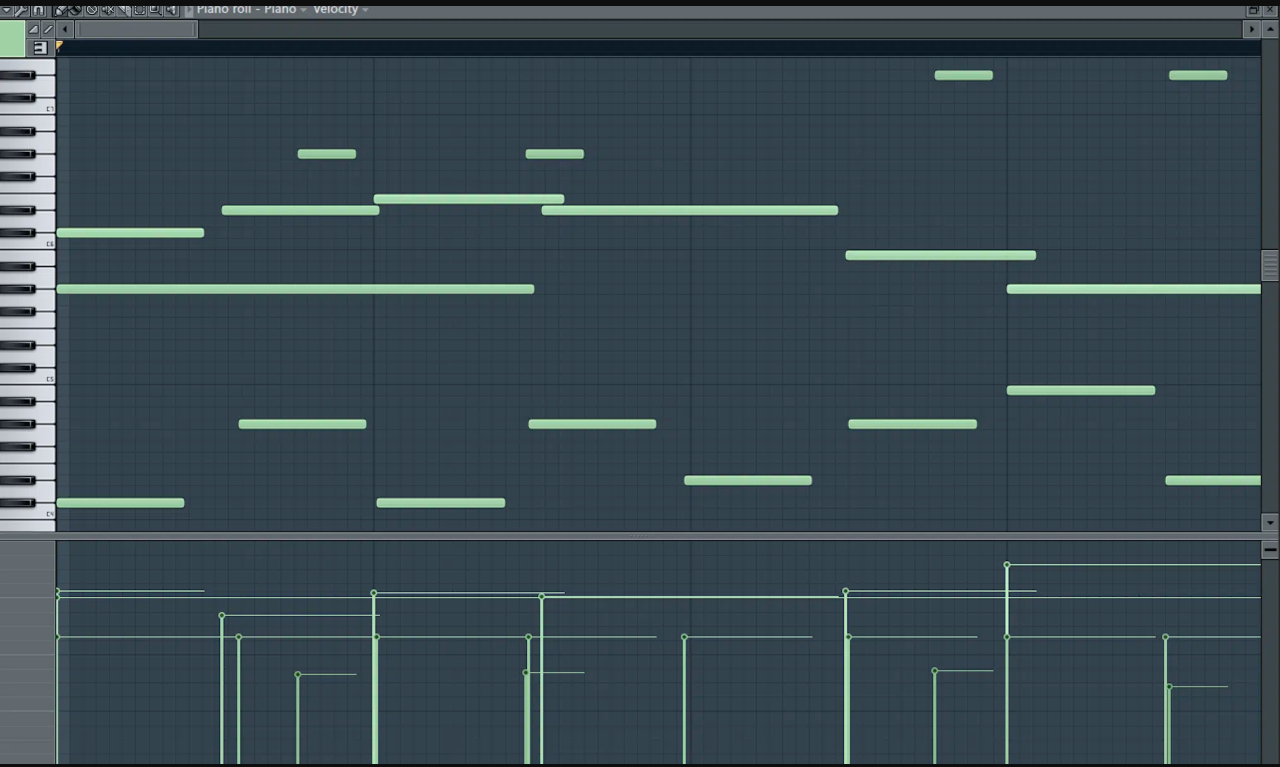
\includegraphics[scale=0.25]{piano-roll.png} 
\end{frame}



\subsubsection*{DFA}
\begin{frame}{Análisis de Fluctuación sin Tendencia}
\begin{block}{En general}
\begin{itemize}
\item Aplicamos \textbf{técnicas de series temporales}
\item \textit{Espacio de fases} y \textit{sistema subyacente}
\begin{itemize}
\item Herramientas matemáticas y estadísticas
\item \textbf{\textit{DFA}} y \textbf{\textit{Exponente de Hurts}}
\end{itemize}
\end{itemize}
\end{block}
\centering
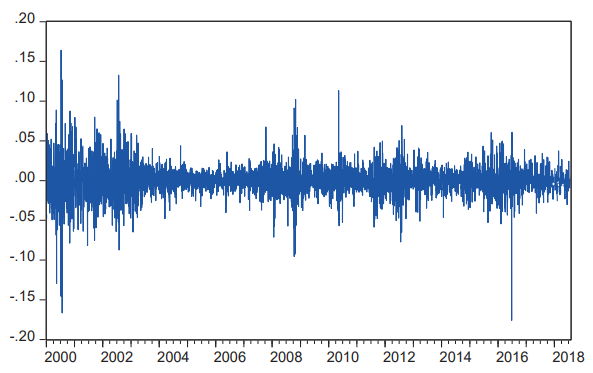
\includegraphics[scale=0.4]{idea-grafica.png} 
\end{frame}

\subsection{Antecedentes de la metología}

\begin{frame}{Antecedentes}
\begin{block}{Artículos revisados}
\begin{itemize}
\item Jennings et al. (2003) aplicaron \textbf{DFA} sobre la \textit{sonoridad} (estimada como la varianza local de la amplitud) en 90 canciones de \textit{9 géneros musicales.}
\item González-Espinoza et al (2017) analiza 304 partituras MIDI de \textit{7 compositores clásicos} usando \textbf{DFA} y su versión modificada (MDFA)
\end{itemize}
\end{block}

\end{frame}

\begin{frame}{Variance fluctuations in nonstationary time series: a comparative study of music genres (2003)}
\begin{block}{En general}
Encontraron que géneros como WECT (Western European Classical Tradition) presentan mayor complejidad temporal, mientras que géneros bailables como el Techno-dance muestran patrones más periódicos y predecibles.
\end{block}
\begin{block}{Géneros analizados}
\begin{multicols}{2}
\begin{enumerate}
\item Forró
\item Techno-dance
\item Brazilian Pop
\item Rock and Roll
\item Jazz
\item Javanese
\item New Age
\item Hindustani
\item WECT
\end{enumerate}
\end{multicols}
\end{block}
\end{frame}

\begin{frame}{Multiple scaling behaviour and nonlinear traits in music scores (2017)}
\small
\begin{block}{En general}
\begin{itemize}
\item Identifica distintos perfiles de correlación que caracterizan la dinámica compositiva de cada autor
\item Demuestra que existen patrones no lineales específicos de cada compositor que podrían influir en la percepción estética de la música.
\end{itemize}
\end{block}
\begin{block}{Compositores analizados}
\begin{multicols}{2}
\begin{itemize}
\item \textbf{Palestrina:} 21 piezas
\item \textbf{Bach:} 63 piezas
\item \textbf{Haydn:} 48 piezas
\item \textbf{Mozart:} 36 piezas
\item \textbf{Beethoven:} 63 piezas
\item \textbf{Dvořák:} 25 piezas
\item \textbf{Shostakovich:} 48 piezas
\end{itemize}
\end{multicols}
\end{block}
\end{frame}
\section{Métodos y Materiales}
\subsection{Enfoque propuesto}
\begin{frame}
\tableofcontents[currentsection] % Solo muestra la sección actual
\end{frame}

\begin{frame}{Nuestra aportación}
\begin{block}{Proponemos}
\begin{itemize}
\item Normalizaciones y segmentaciones con respecto a \textit{semidifusas} de las canciones
\end{itemize}
\end{block}
\centering
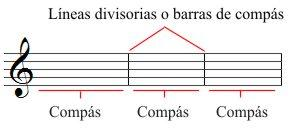
\includegraphics[scale=0.6]{Compas.jpg} 
\end{frame}

\begin{frame}{Idea gráfica}
\centering
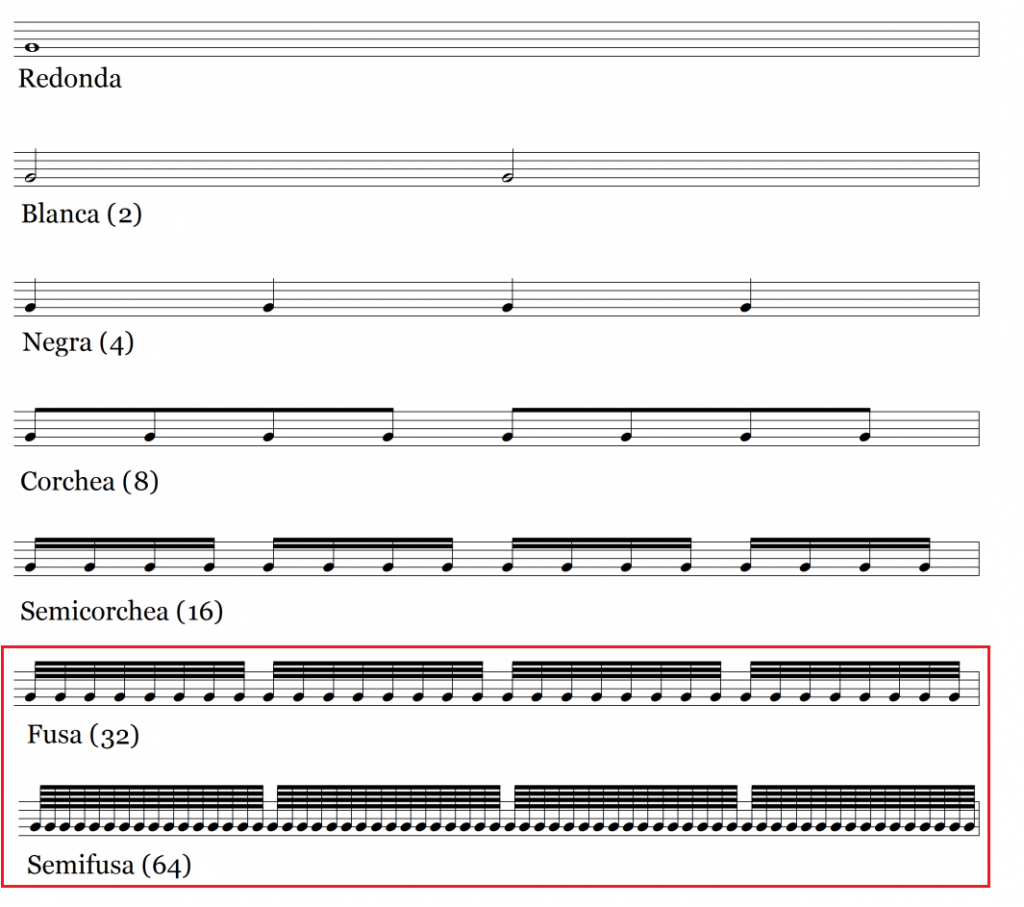
\includegraphics[scale=0.23]{semidifusa.png} 
\end{frame}

\subsection{Programas desarrollados}


\begin{frame}{Objetivos}
\begin{block}{Busqueda de canciones}
\begin{itemize}
\item \texttt{busca-gen-id.py}
\item \texttt{tracsxid.py}
\end{itemize}
\end{block}
\begin{block}{Tratamiento de los datos}
\begin{itemize}
\item \texttt{midi-csv.py}  
\end{itemize}
\end{block}
\begin{block}{Analisis de Fluctuación sin Tendencia}
\begin{itemize}
\item \texttt{resultados-aft} 
\end{itemize}
\end{block}
\end{frame}

\section{Resultados y discusión}
\subsection{Base de datos}
\begin{frame}
\tableofcontents[currentsection] % Solo muestra la sección actual
\end{frame}

\begin{frame}{}


\small

\begin{tabular}{lcc}
\toprule
\textbf{Canción} & \textbf{Semidifusas} & \textbf{Instrumentos} \\
\midrule
Frankie Ruiz – La Cura & 24,573 & 7 \\
The Latin Brothers – Patrona de los Reclusos & 24,303 & 5 \\
Luis Enrique – Compréndelo & 22,589 & 6 \\
Richie Ray – Agúzate & 22,200 & 4 \\
The Latin Brothers – La Guayaba & 20,736 & 3 \\
Celia Cruz – Toro Mata & 19,283 & 5 \\
Héctor Lavoe – Déjala que Siga & 18,242 & 6 \\
El Gran Combo – La Loma del Tamarindo & 16,847 & 8 \\
Orquesta Guayacán – Un Vestido Bonito & 16,257 & 7 \\
Rubén Blades – Pedro Navaja & 14,490 & 6 \\
Jerry Rivera – Amores como el Nuestro & 14,458 & 6 \\
Frankie Ruiz – Amor de un Momento & 14,348 & 7 \\
El Gran Combo – Me Liberé & 13,810 & 6 \\
Frankie Ruiz – Quiero Llenarte & 13,751 & 6 \\
The Latin Brothers – Sobre las Olas & 13,744 & 7 \\
\bottomrule
\end{tabular}

\end{frame}

\subsection{Gráficas}

\begin{frame}{De música a datos}
\begin{block}{Ejemplo concreto}
\textbf{Héctor Lavoe} - Déjala que siga
\end{block}
\centering
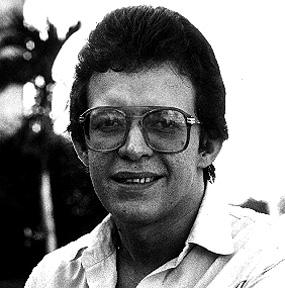
\includegraphics[scale=0.5]{hector_lavoe.jpg} 
\end{frame}

\begin{frame}{\textbf{Héctor Lavoe} - Déjala que siga}
\centering
\begin{minipage}{0.48\textwidth}
    \centering
    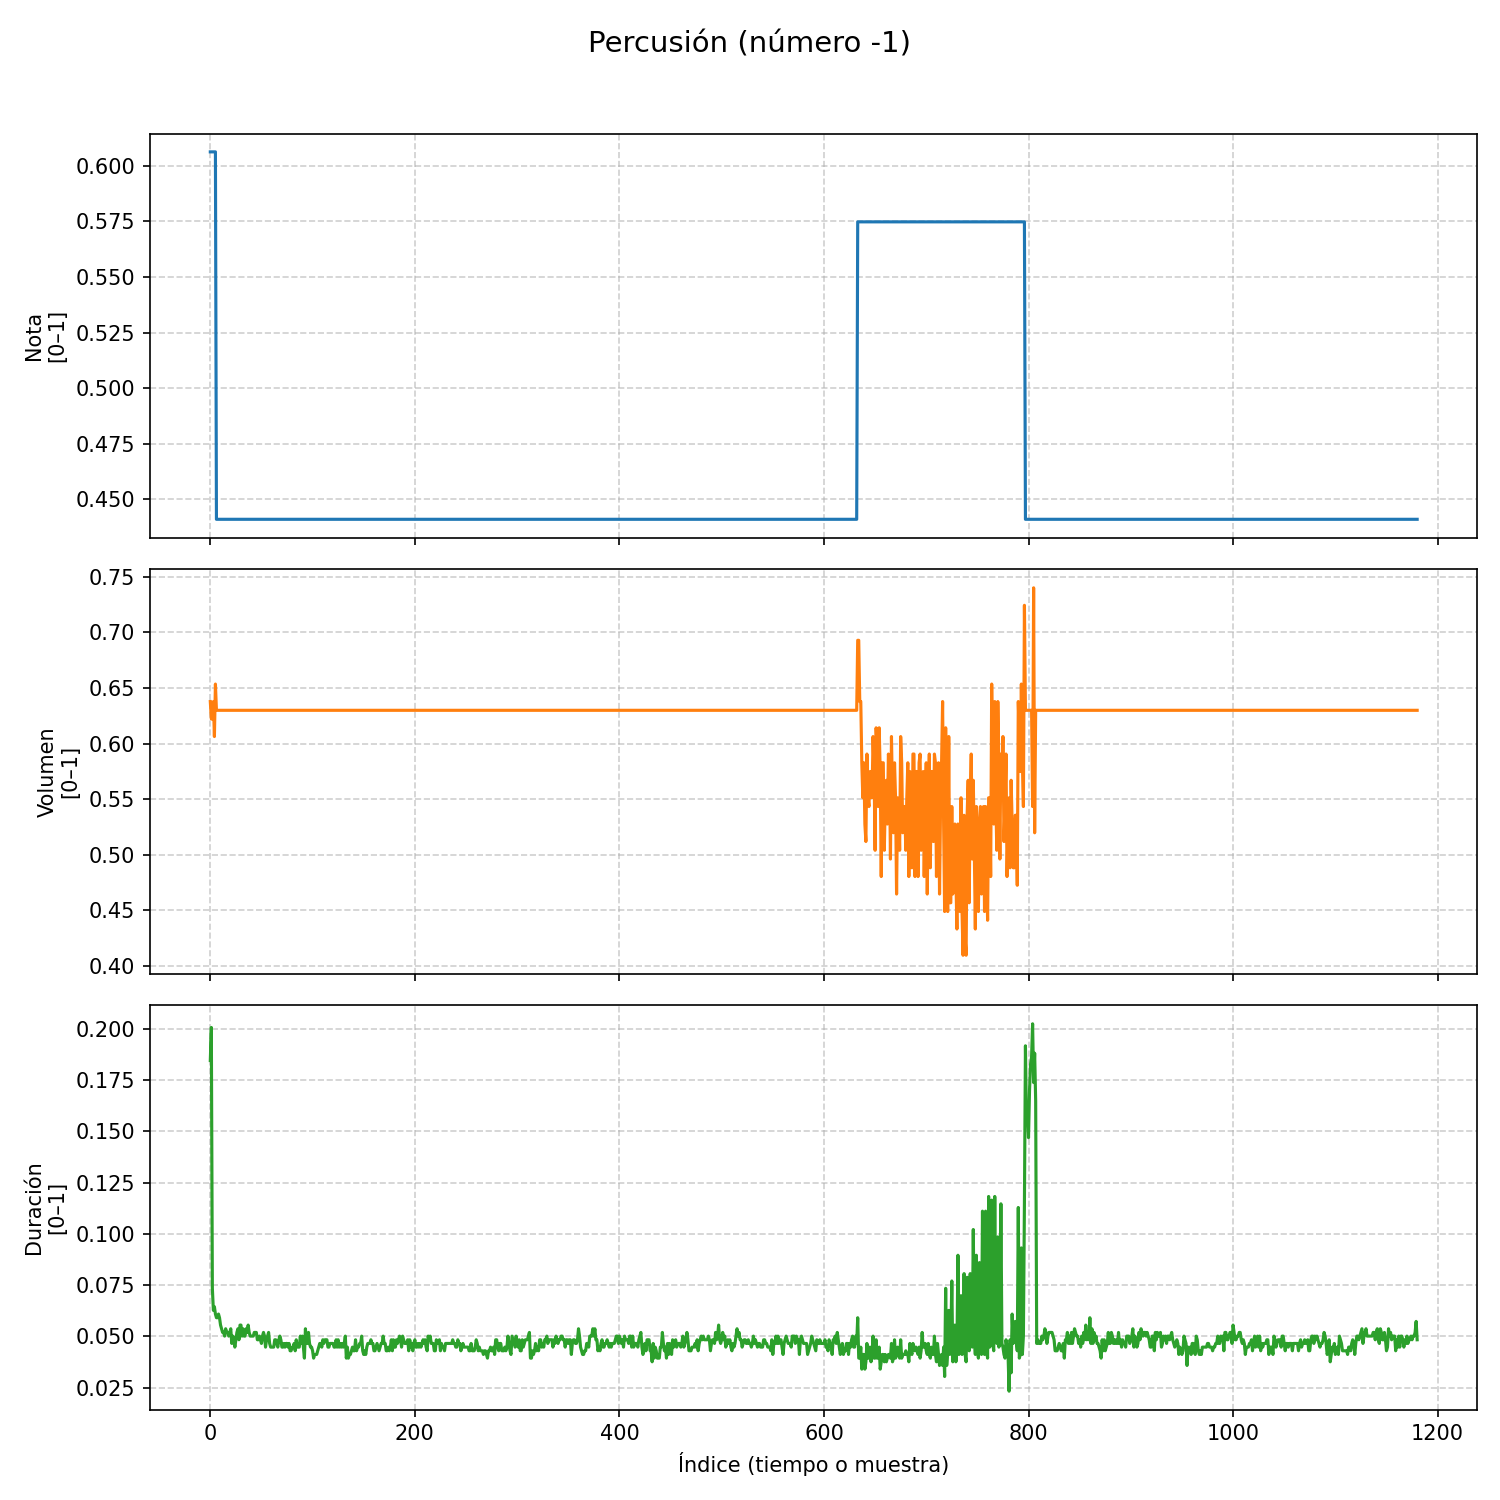
\includegraphics[scale=0.3]{-1_Percusion.png} 
\end{minipage}
\hfill
\begin{minipage}{0.28\textwidth}
    \centering
    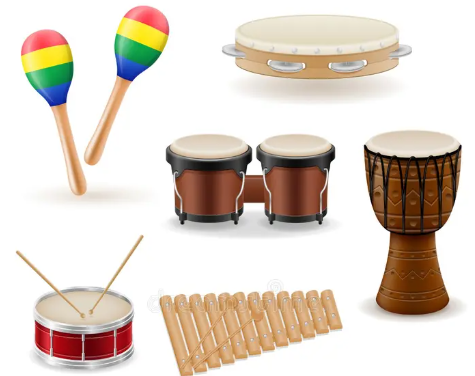
\includegraphics[scale=0.1]{perc.png}
\end{minipage}
\end{frame}

\begin{frame}{\textbf{Héctor Lavoe} - Déjala que siga}
\centering
\begin{minipage}{0.48\textwidth}
    \centering
    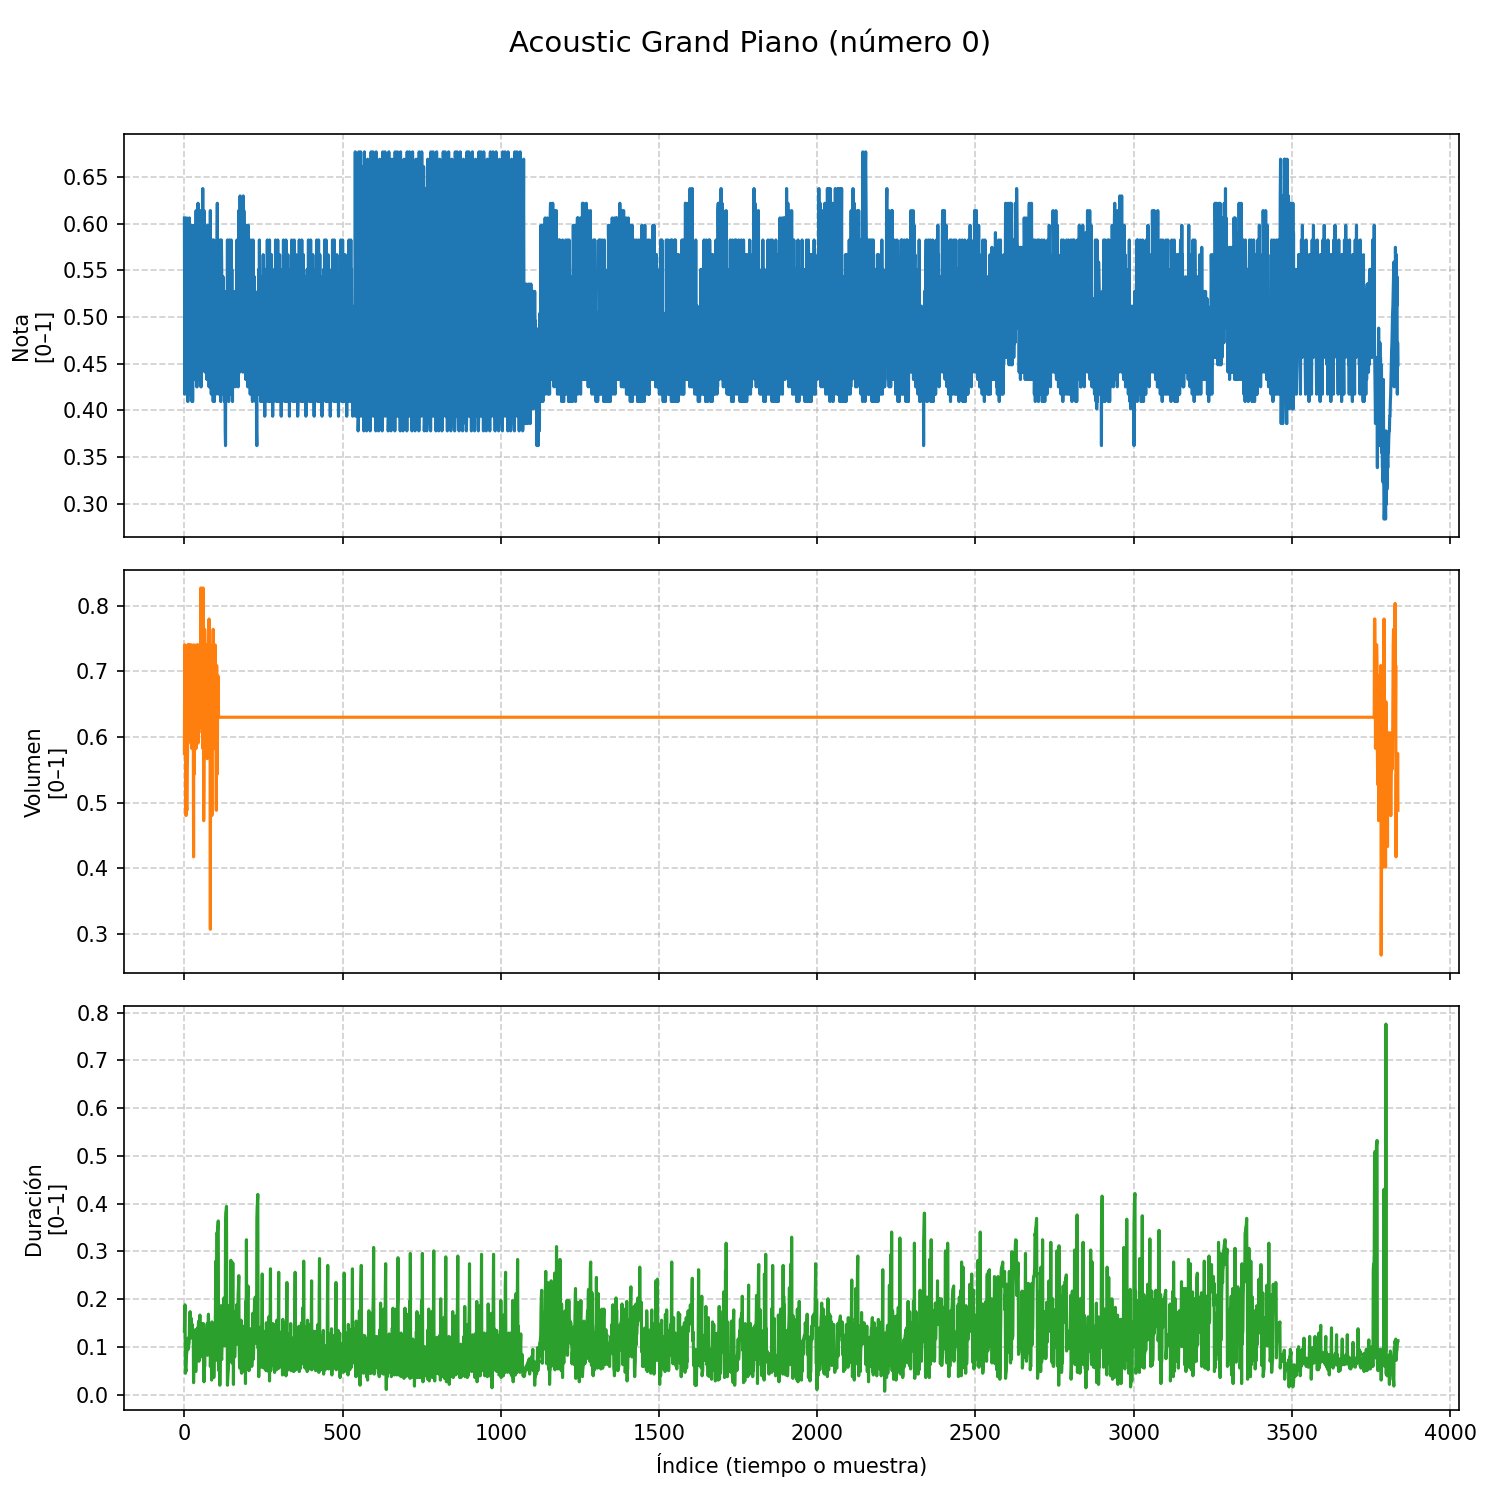
\includegraphics[scale=0.3]{0_Acoustic_Grand_Piano.png} 
\end{minipage}
\hfill
\begin{minipage}{0.28\textwidth}
    \centering
    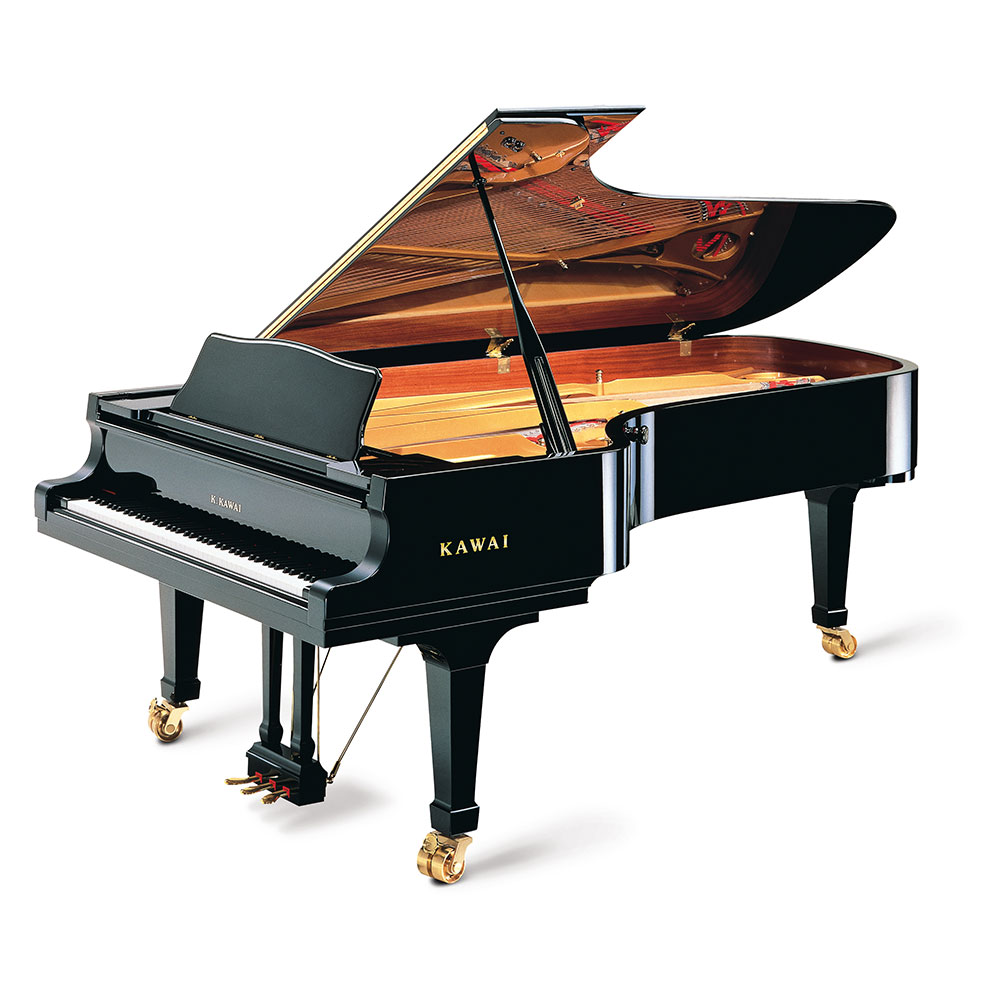
\includegraphics[scale=0.1]{piano.jpg}
\end{minipage}
\end{frame}

\begin{frame}{\textbf{Héctor Lavoe} - Déjala que siga}
\centering
\begin{minipage}{0.48\textwidth}
    \centering
    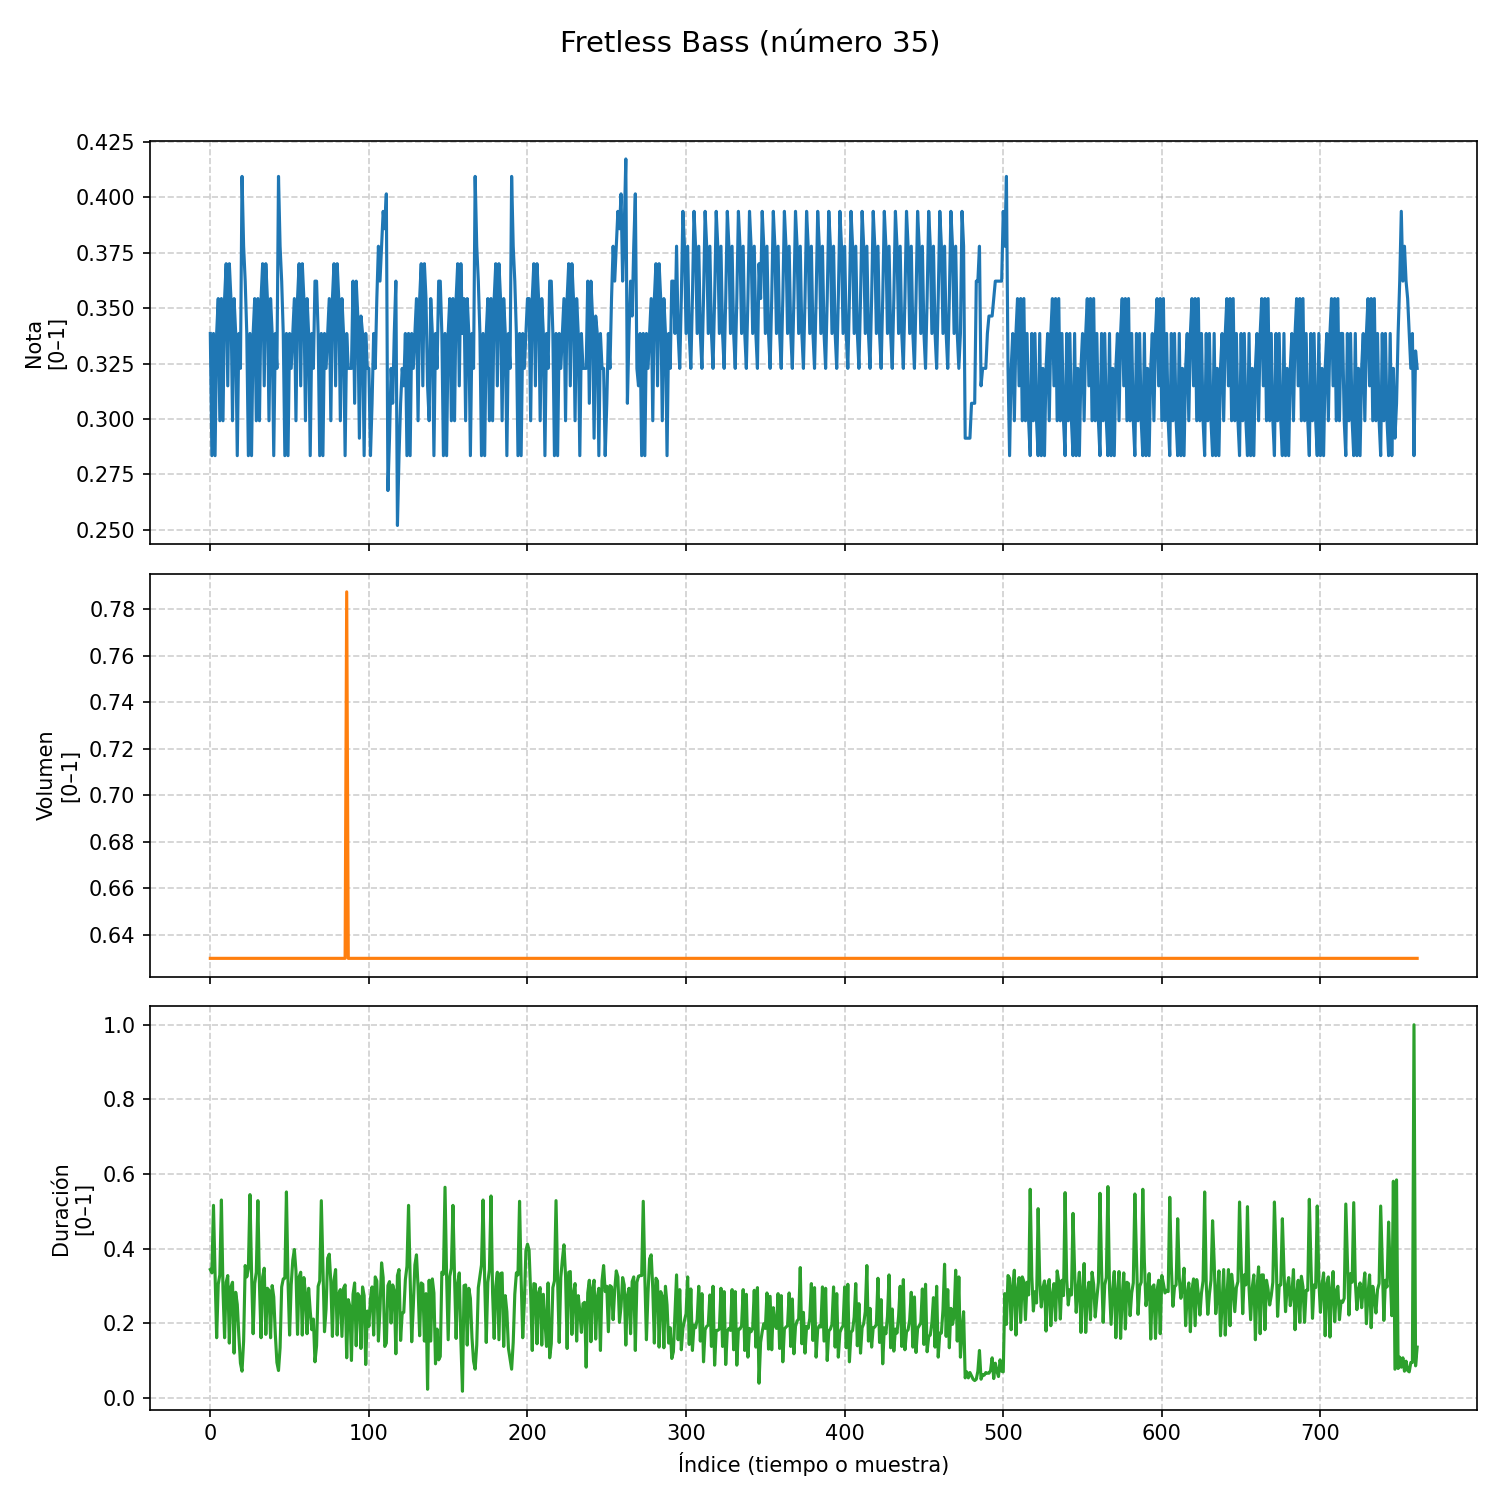
\includegraphics[scale=0.3]{35_Fretless_Bass.png} 
\end{minipage}
\hfill
\begin{minipage}{0.28\textwidth}
    \centering
    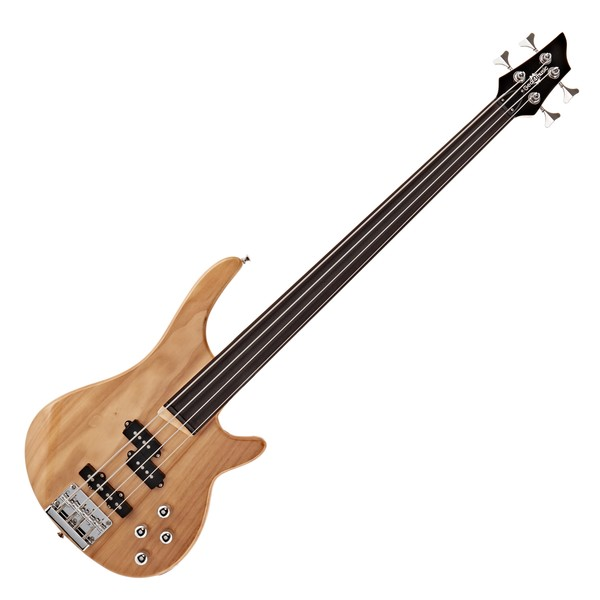
\includegraphics[scale=0.1]{fretless-bajo.jpg}
\end{minipage}
\end{frame}

\begin{frame}{\textbf{Héctor Lavoe} - Déjala que siga}
\centering
\begin{minipage}{0.48\textwidth}
    \centering
    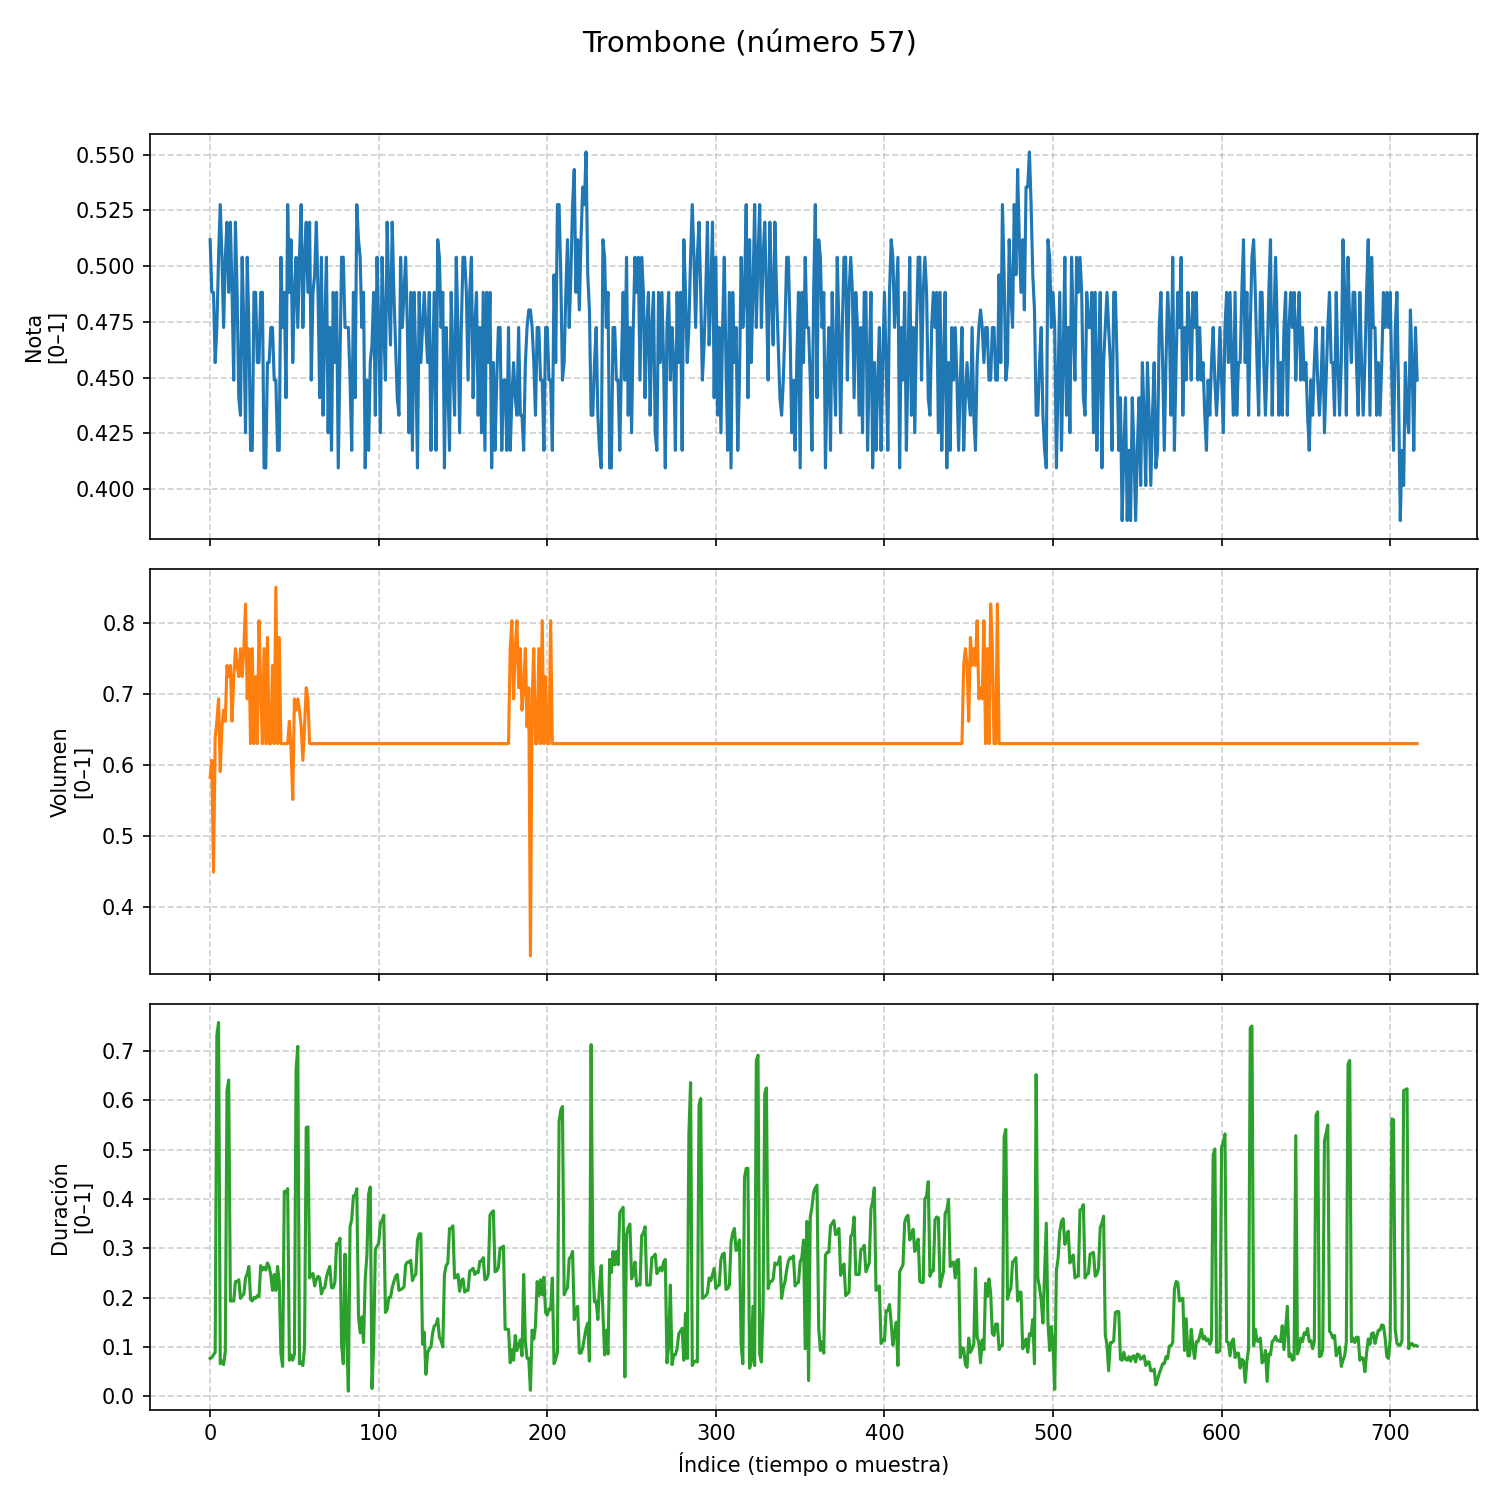
\includegraphics[scale=0.3]{57_Trombone.png}  
\end{minipage}
\hfill
\begin{minipage}{0.28\textwidth}
    \centering
    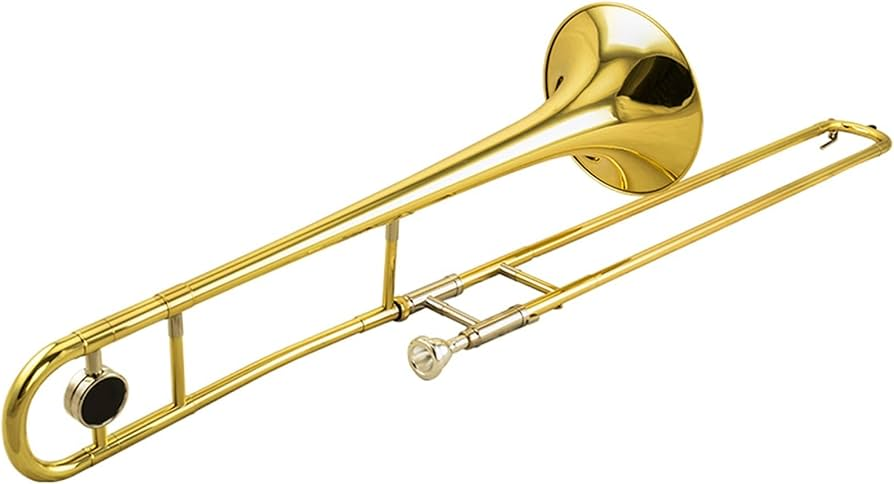
\includegraphics[scale=0.1]{trombone.jpg}
\end{minipage}
\end{frame}


\begin{frame}{Promedios de Fluctuaciones}
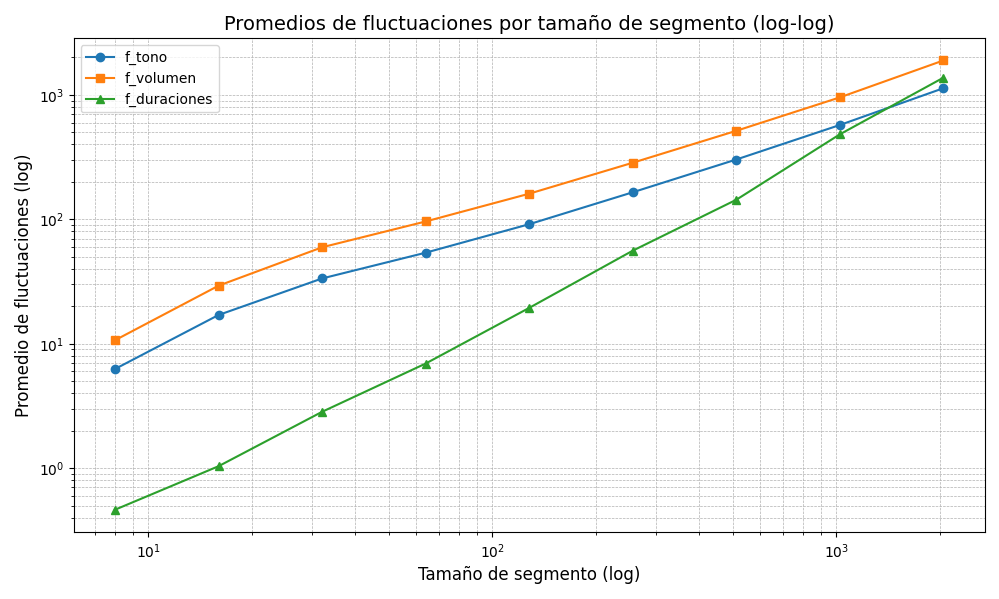
\includegraphics[scale=0.4]{promedios_fluctuaciones.png} 
\end{frame}

\subsection{Exponentes}
\begin{frame}{Interpretación directa del exponente \(\alpha\) en el análisis DFA}
\begin{table}[h!]
\centering
\small
\renewcommand{\arraystretch}{1.3}
\begin{tabular}{lcc}
\hline
\textbf{Variable} & \(\boldsymbol{\alpha}\) & \textbf{Interpretación} \\ 
\hline
Tono      & 0.886 & Persistente\\ 
Volumen   & 0.879 & Persistente\\ 
Duración  & 1.451 & Persistente \\ 
\hline
\end{tabular}
\caption{El exponente \(\alpha\) proviene de la relación \(\langle v^{(k)}(\tau)\rangle \propto \tau^{2\alpha}\).}
\end{table}
\end{frame}

\begin{frame}{Resultados del análisis DFA}
\begin{table}[h!]
\centering
\small
\renewcommand{\arraystretch}{1.3}
\begin{tabular}{lccc}
\hline
\small
\textbf{Variable} & \(\boldsymbol{\alpha}\) & \(\boldsymbol{H_x = \alpha - 1}\) & \textbf{Interpretación} \\ 
\hline
Tono      & 0.886 & -0.114 & Anti-persistente \\ 
Volumen   & 0.879 & -0.121 & Anti-persistente \\ 
Duración  & 1.451 & 0.451  & Anti-persistente \\ 
\hline
\end{tabular}
\caption{Exponentes de Hurst obtenidos tras integración previa (\(y(t) = \int [x(t') - \bar{x}]dt'\)).}
\end{table}
\end{frame}

\begin{frame}{Referencias}
\tiny
\begin{thebibliography}{99}

\bibitem{kantz2003}
H. Kantz and T. Schreiber, \textit{Nonlinear Time Series Analysis}, 2nd ed. Cambridge, U.K.: Cambridge University Press, 2003.

\bibitem{jennings2003}
H. D. Jennings, P. Ch. Ivanov, A. M. Martins, P. C. da Silva, and G. M. Viswanathan, “Variance fluctuations in nonstationary time series: a comparative study of music genres,” \textit{arXiv preprint cond-mat/0312380v3}, Dec. 2003. [Online]. Available: \url{https://arxiv.org/abs/cond-mat/0312380v3}

\bibitem{gonzalez2017}
A. González-Espinoza, H. Larralde, G. Martínez-Mekler, and M. Müller, “Multiple scaling behaviour and nonlinear traits in music scores,” \textit{R. Soc. Open Sci.}, vol. 4, no. 12, p. 171282, 2017. [Online]. Available: \url{https://doi.org/10.1098/rsos.171282}

\bibitem{musicbrainzDB}
“MusicBrainz Database.” [Online]. Available: https://musicbrainz.org/doc/MusicBrainz_Database. [Accessed: Oct. 21, 2025].

\bibitem{artsmusica_figuras}
“Las figuras musicales y sus valores rítmicos,” ArtsMúsica. [Online]. Available: https://www.artsmusica.net/teoria-musical/las-figuras-musicales-y-sus-valores-ritmicos/. [Accessed: Oct. 21, 2025].


\end{thebibliography}

\end{frame}

\subsubsection*{Agradecimientos}
\begin{frame}{}
\begin{block}{Se agradece profundamente}
\begin{itemize}
\item Sociedad Matemática Mexicana
\item El capítulo estudiantíl afiliado a la SMM \textbf{\textit{Transformados por Laplace}}
\item \textbf{Director de Tesis:} Dr. José L. Herrera-Aguilar
\end{itemize}

\end{block}
\end{frame}

\subsection{Preguntas}
\begin{frame}{Muchas gracias por su atención}
\centering
\begin{Huge}
\textbf{Preguntas}
\end{Huge}
\end{frame}






\section*{Detalles técnicos}
\subsection*{Diegramas de flujo}
\subsubsection*{Búsqueda de canciones y recolección de MIDIs}
\begin{frame}{\textit{busca-gen-id.py}}
\centering
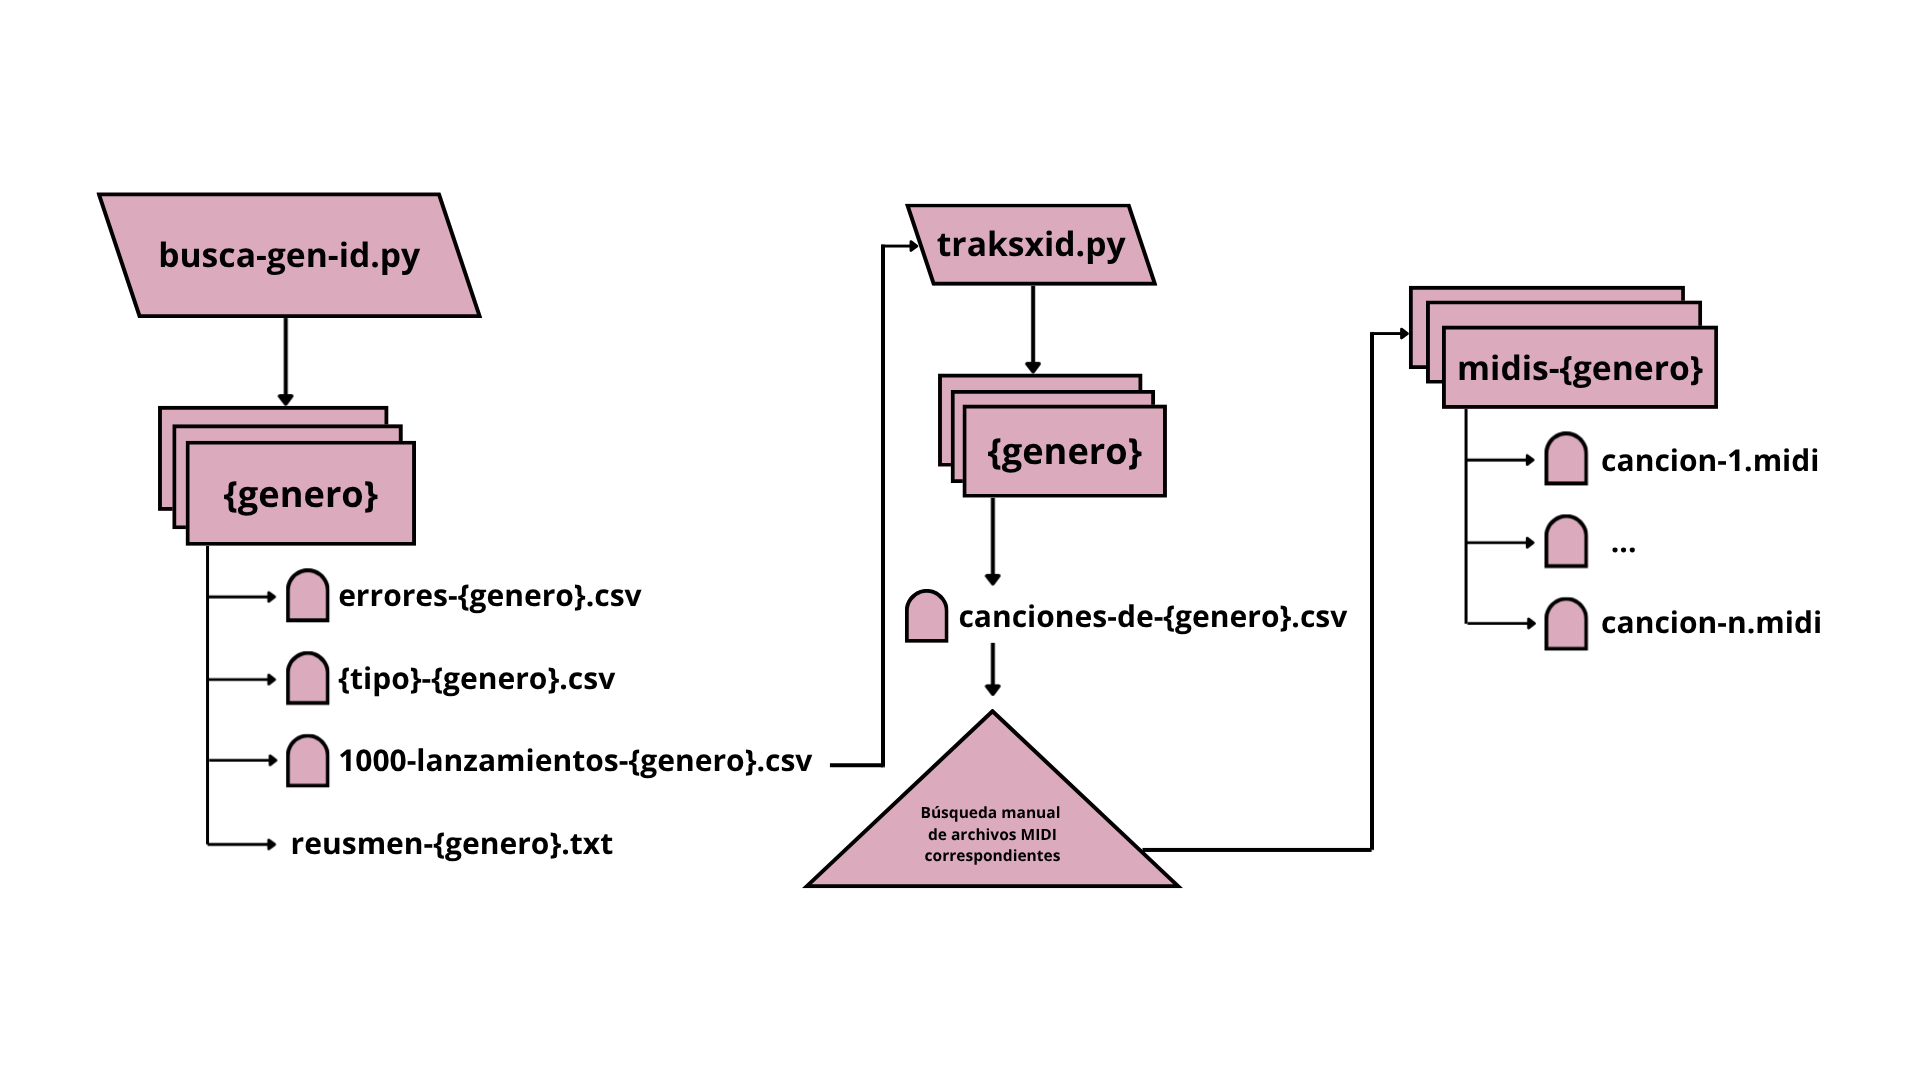
\includegraphics[scale=0.22]{busca-gen-id.png} 
\end{frame}
\subsubsection*{Fabricación de series temporales}
\begin{frame}{\textit{midis-csv.py}}
\centering
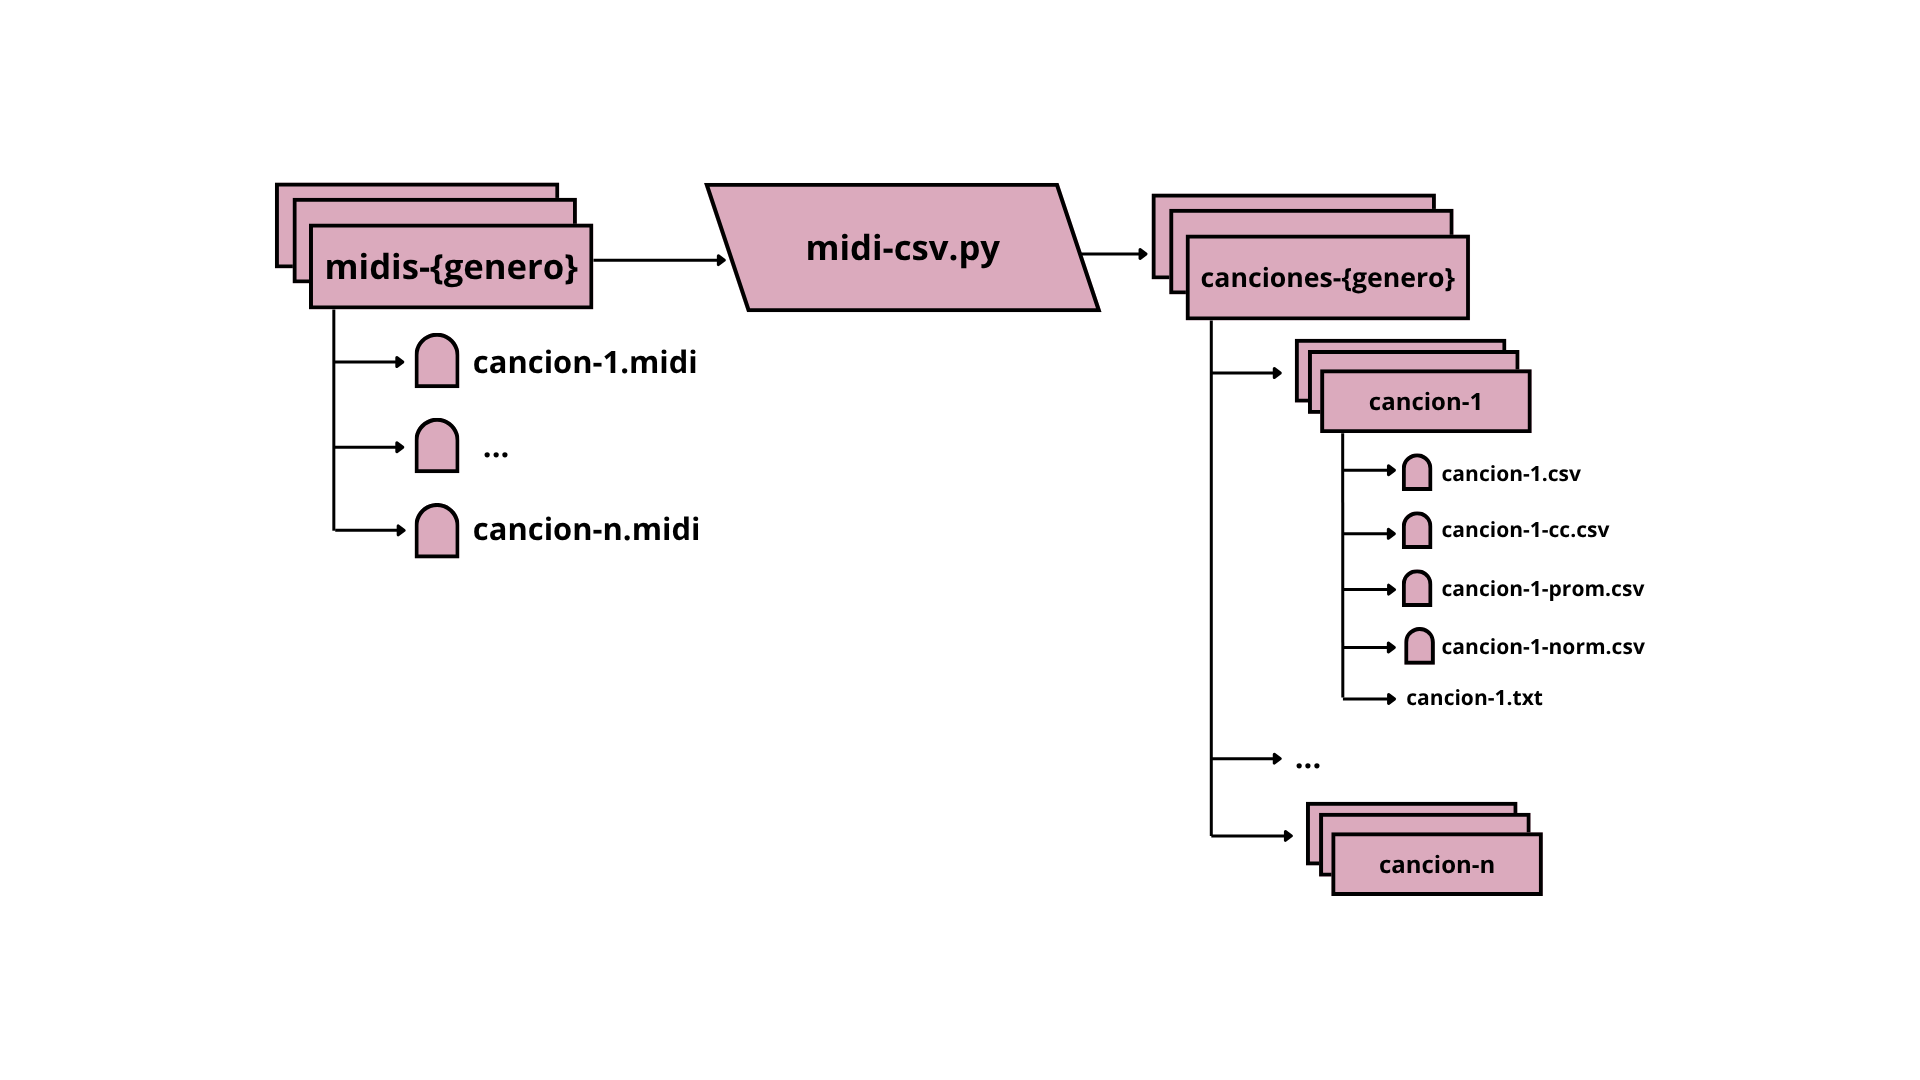
\includegraphics[scale=0.25]{midi-csv.png} 
\end{frame}
\subsubsection*{Análisis de Fluctuación sin tendencia}
\begin{frame}{\textit{aft.c}}
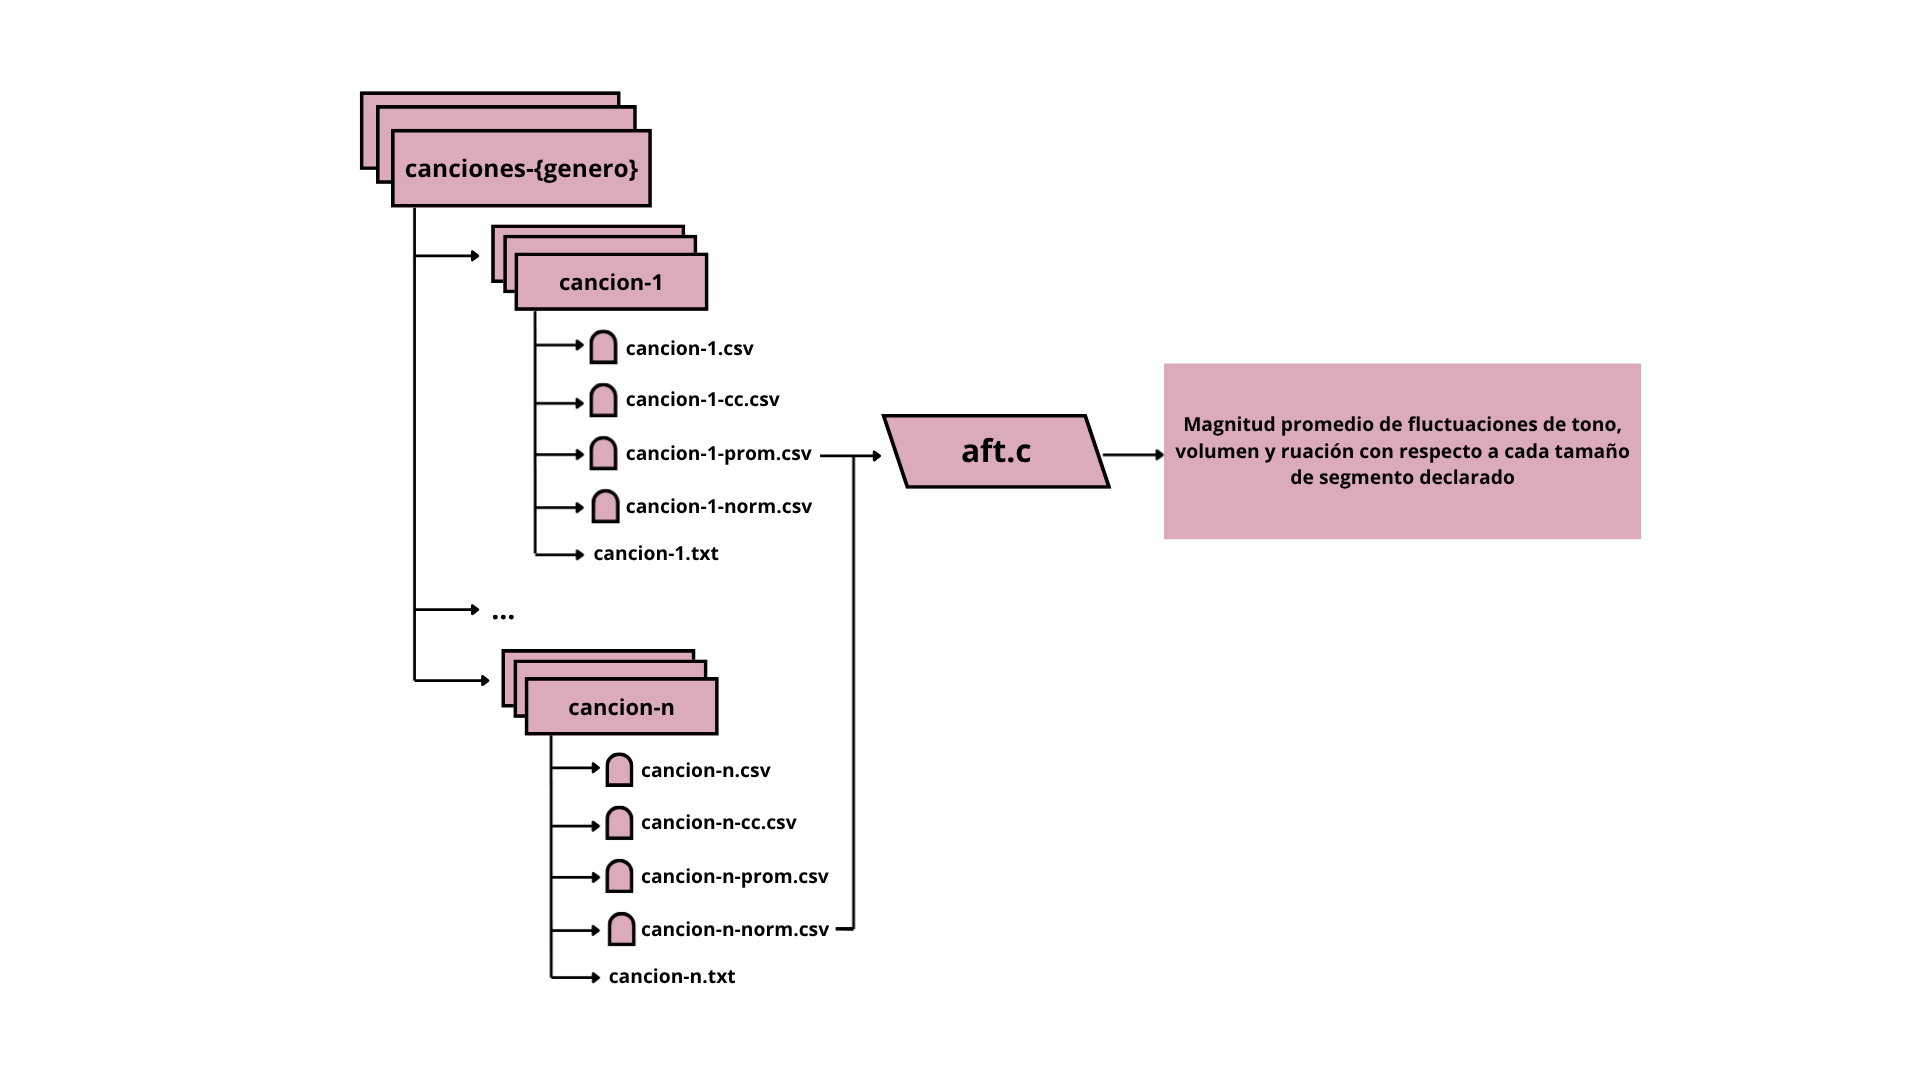
\includegraphics[scale=0.25]{pruebas-resultados.png} 
\end{frame}

\subsection*{DFA}
\subsubsection*{Terminos relacionados}
\begin{frame}{Términos relacionados}
\begin{block}{Autosimilitud}
Una señal o figura es \textit{autosimilar} si luce igual bajo una transformación de escala \textbf{igual} en todos los ejes.
\end{block}

\begin{block}{Autoafinidad}
Una señal es \textit{autoafín} si luce igual bajo una transformación \textbf{desigual} de escala en cada eje. La forma se conserva estadísticamente si se escala de la forma:

\begin{equation}
\langle \Delta x^2 \rangle \propto \Delta t^{2H},
\end{equation}

donde al exponente $H$ le llamamos \textbf{\textit{exponente de Hurst.}}
\end{block}
\subsubsection*{Exponente de Hurst}
\end{frame}

\begin{frame}{Exponente de Hurst}
\begin{block}{En general}
\begin{itemize}
	\item Es un número entre 0 y 1 que caracteriza el grado de dependencia temporal 
	\item Nos dice qué tan correlacionados están los cambios a través del tiempo
	\item Indica cómo crece la varianza de los incrementos $(x(t+\Delta t)-x(t))^2$ al aumentar $\Delta t$.
	
\end{itemize}
\medskip
$$
\langle \Delta x^2 \rangle \propto \Delta t^{2H}
$$
\end{block}
\end{frame}

\subsubsection*{Paso a paso}
\begin{frame}{\textbf{DFA} Paso a paso (1/3)}
\begin{block}{\textbf{Paso 1} Construir la señal integrada}
Primero se transforma la señal original $x(t)$ en una \textit{señal acumulativa} o 'camino integrado'
\begin{equation}
y(t) = \int_{0}^{t} (x(t') - \bar{x}) dt',
\end{equation}
\end{block}
\end{frame}

\begin{frame}{\textbf{DFA} Paso a paso (2/3)}
\begin{block}{\textbf{Paso 2} Dividir en ventanas y eliminar la tendencia local}
Se divide la señal integrada $y(t)$ en ventanas de longitud $\tau$ y en cada ventana se ajusta un polinomio de grado $k$ que representa la \textit{tendencia local} $g^{(k)}(t)$

Esa tendencia se resta para obtener las fluctuaciones sin tendencia
\begin{equation}
v^{(k)}(\tau)=\text{RMS}[y(t)-g^{(k)}(t)]
\end{equation}

Donde \textit{RMS} es la raíz cuadrada del promedio cuadrático de los residuos.
\end{block}

\end{frame}


\begin{frame}{\textbf{DFA} Paso a paso (3/3)}
\begin{block}{\textbf{Paso 3} Escalamiento de la fluctuación}
Después se calcula cómo crece esa fluctuación $v^{(k)}(\tau)$ con el tamaño de ventana $\tau$
\begin{equation}
\langle v^{(k)}(\tau) \rangle \propto \tau^{2+2H}
\end{equation}
Este crecimiento es el que da el \textbf{\textit{exponente de Hurst}}
\end{block}
\end{frame}


\end{document}


